\documentclass[11pt,letterpaper]{article}
\usepackage[T1]{fontenc}
\usepackage{lmodern,microtype}
\usepackage[margin=1in,headheight=15pt]{geometry}
\usepackage{amsmath,amssymb,amsthm,mathtools}
\usepackage{booktabs,tabularx,graphicx,xcolor,fancyhdr,enumitem}
\usepackage{xurl}
\usepackage[colorlinks=true,linkcolor=teal!65!black,citecolor=teal!65!black,urlcolor=teal!65!black]{hyperref}
\newtheorem{theorem}{Theorem}[section]
\newtheorem{lemma}[theorem]{Lemma}
\newtheorem{proposition}[theorem]{Proposition}
\newtheorem{corollary}[theorem]{Corollary}
\theoremstyle{definition}
\newtheorem{definition}[theorem]{Definition}
\theoremstyle{remark}
\newtheorem{remark}[theorem]{Remark}
\newcommand{\F}{\mathbb F}
\newcommand{\E}{\mathbb E}
\newcommand{\Prob}{\mathbb P}
\newcommand{\TV}{d_{\mathrm{TV}}}
\newcommand{\Law}{\mathcal L}
\newcommand{\rank}{\operatorname{rank}}
\newcommand{\rad}{\operatorname{rad}}
\newcommand{\nul}{\operatorname{nullity}}
\newcommand{\Sp}{\operatorname{Sp}}
\newcommand{\Emb}{\operatorname{Emb}}
\newcommand{\Mat}{\operatorname{Mat}}
\newcommand{\qb}[2]{\genfrac{[}{]}{0pt}{}{#1}{#2}_{q}}
\newcommand{\abs}[1]{\lvert #1\rvert}
\newcommand{\pin}{6d284fcf75bc3a91bb2e79ba7636f94724bff62c}
\setlength{\emergencystretch}{3em}
\setlength{\parskip}{3pt}
\setlist{topsep=5pt,itemsep=3pt}
\pagestyle{fancy}
\fancyhf{}
\fancyhead[L]{\small Hidden dependence in symplectic observations}
\fancyhead[R]{\small 27 November 2026}
\fancyfoot[C]{\thepage}
\hypersetup{pdftitle={Hidden higher-order dependence in symplectic observations},pdfauthor={Research note prepared for Vladimir Reshetnikov}}
\title{\textbf{Hidden higher-order dependence\\in symplectic observations}\\[6pt]
\large Exact joint laws and a sharp total-dimension threshold}
\author{Research note prepared for Vladimir Reshetnikov}
\date{27 November 2026}

\begin{document}
\maketitle
\begin{abstract}
The symplectic compression theory in the ProveIt GRH project gives detailed laws for an observation between two frames. We extend it to the complete set of pairings among any number of independent frames, allowing arbitrary prescribed alternating forms on the individual frames and every finite-field characteristic. We prove an exact joint likelihood, a constructive minimum ambient dimension, and explicit total-variation bounds with a transition at total frame dimension equal to ambient dimension. The proof of the upper bound retains only injective combined realizations and controls their missing likelihood by one exact kernel moment.

The resulting dependence phenomenon is strong. For every fixed number $k\ge3$, there are natural observations whose every proper frame marginal is exponentially close to independent uniform entries, while their full joint law is exponentially close to perfectly distinguishable from that model. Observations indexed by a forest are exactly independent. In particular, three $40\times40$ binary matrices constructed from random isotropic frames in dimension $100$ are pairwise independent, each is within $1.59\cdot10^{-6}$ of uniform, and their joint distance from three independent uniform matrices exceeds $0.99999809$. All results are unconditional finite linear algebra. The packet contains complete proofs and exact computational checks; it is not a Lean formalization.
\end{abstract}

\section{The result and its place in the source project}

\subsection{A concrete statement}

Let $V=\F_2^{100}$ carry a nondegenerate alternating pairing $\langle\cdot,\cdot\rangle$. Choose independently and uniformly three ordered lists $X_1,X_2,X_3$, each consisting of $40$ linearly independent vectors whose pairings within the list are all zero. Record the three matrices
\[
 M_{12}=X_1^{\mathsf T}JX_2,\qquad
 M_{13}=X_1^{\mathsf T}JX_3,\qquad
 M_{23}=X_2^{\mathsf T}JX_3,
\]
where $J$ represents the pairing. Write $U$ for a $40\times40$ matrix of independent fair bits.

\begin{theorem}[Three almost uniform matrices with hidden joint dependence]\label{thm:headline}
The three matrix-valued random variables $M_{12},M_{13},M_{23}$ are pairwise independent exactly. Each satisfies
\begin{equation}\label{eq:headline-one}
 \TV(\Law(M_{ij}),\Law(U))
 <\frac{5}{3}\,2^{-20}<1.59\cdot10^{-6}.
\end{equation}
Nevertheless, for three independent copies $U_1,U_2,U_3$,
\begin{equation}\label{eq:headline-all}
 \TV\bigl(\Law(M_{12},M_{13},M_{23}),\Law(U_1,U_2,U_3)\bigr)
 >0.99999809.
\end{equation}
The joint distance from the product of the three actual marginal laws exceeds $0.99999332$ as well. Thus the effect persists after all marginal biases are matched exactly.
\end{theorem}

Total variation is $\TV(P,Q)=\sup_A\abs{P(A)-Q(A)}$. It measures the largest difference in the probability of the same event under the two models. The separating event here is particularly simple: assemble the $120\times120$ matrix
\begin{equation}\label{eq:triangle-gram}
 \Gamma=\begin{pmatrix}
 0&M_{12}&M_{13}\\
 -M_{12}^{\mathsf T}&0&M_{23}\\
 -M_{13}^{\mathsf T}&-M_{23}^{\mathsf T}&0
 \end{pmatrix}
 \quad\hbox{and test whether }\rank\Gamma\le100.
\end{equation}
For the constructed matrices the test always accepts. For independent uniform blocks it accepts with probability less than $0.00000191$. Signs in \eqref{eq:triangle-gram} become plus signs in characteristic two; its diagonal remains zero.

\subsection{What is inherited and what is extended}

The source is the directory \texttt{Analysis/GeneralizedRiemannHypothesis} in ProveIt at commit
\begin{center}\small\texttt{\pin}.\end{center}
Its README describes a consolidated article from $142$ reports, with $42$ further research packets placed but not yet merged. At this snapshot, ten additional archives remain in its incoming directory. The article's inventory reports $997$ theorem-like results; the merge itself is explicitly distinguished from independent verification \cite{ProveIt}.

We used the full section inventory, examined the source-mechanism section and the frame-statistics section, and compared the relevant newer two-frame reports. The immediate starting points are the article labels \texttt{spn:thm:complete-law} (the exact two-frame law), \texttt{spn:lem:alt-gram}, and the correlated-observation question under \texttt{spn:q:symplectic}. The source-mechanism section links this branch of the project to its second-moment spanning lemmas and positive-type matrix estimates. The present work extends that finite model.

\begin{center}\small
\begin{tabularx}{\linewidth}{@{}p{.28\linewidth}XX@{}}
\toprule
Topic & Inspected source & Present contribution\\
\midrule
Exact likelihood & Two prescribed-Gram frames & Any number of frames; one explicit kernel-count polynomial\\
Feasible observations & Two-frame radical-intersection criterion & Minimum dimension for all simultaneous pairings\\
Distributional comparison & Detailed two-frame and residual-form laws & Uniform joint bounds controlled by total frame dimension\\
Correlated observations & Listed as an open direction & Forest independence and dependence invisible in every proper frame marginal\\
\bottomrule
\end{tabularx}
\end{center}

The upstream source exports RH and GRH for Dirichlet $L$-functions. Sutherland's current verification page reports kernel, axiom, and statement checks for the pinned upstream revision \cite{Sutherland}. We inspected that record and the exported statements; we did not rerun the upstream verification. No analytic zero hypothesis enters any proof below.

\paragraph{Novelty assessment.}
The exact results below were not found in the inspected repository material or in the targeted literature search. Random Gram matrices and comparisons with uniform matrix laws have substantial antecedents. Fulman and Goldstein study finite-field rank laws and total variation \cite{FulmanGoldstein}; Li, Li, Qiao, Tao and Wang give a symmetric-Gram comparison over odd fields \cite{LiEtAl}; Farshi and coauthors use finite symplectic matrices in random Clifford circuits \cite{Farshi}; and He proves a cutoff for a different random walk on symplectic forms \cite{He}. The general phenomenon of pairwise independence without joint independence is classical. Our proposed contribution is the exact several-frame theorem and its quantitative hierarchy in this symplectic observation model. This is a supported novelty claim relative to the inspected material, not a certification of worldwide priority.

One incoming archive, \texttt{grh\_uniform\_extensions\_2026-11-27.zip}, was identified but its contents could not be retrieved through the available GitHub interface. The provenance file records that limitation. No assertion of non-overlap with that archive is made.

\section{Setup and main quantitative theorem}

Fix a prime power $q$ and a $2n$-dimensional symplectic space $(V,\langle\cdot,\cdot\rangle)$ over $\F_q$. An alternating form means a bilinear form $H$ with $H(x,x)=0$ for every $x$. This definition includes the diagonal condition in characteristic two.

For $1\le i\le k$, let $E_i$ have dimension $d_i\ge1$ and a prescribed alternating form $H_i$ of rank $2s_i$. Assume
\begin{equation}\label{eq:individual-feasibility}
 d_i-s_i\le n.
\end{equation}
Choose independently and uniformly isometric injections $X_i:(E_i,H_i)\hookrightarrow V$. These are ordered frames; the maps are not identified modulo changes of basis. The individual frames need not have disjoint images. The complete observation consists of
\[
 M_{ij}(u,v)=\langle X_i u,X_j v\rangle\quad(i<j).
\]
Put $E=\bigoplus_iE_i$ and $D=\sum_i d_i$. The observation is equivalently the alternating form $\Gamma$ on $E$ with diagonal blocks $H_i$ and upper off-diagonal blocks $M_{ij}$. Let $\mu$ be its law. Let $\nu$ be the comparison law that keeps the $H_i$ fixed and chooses every entry of every $M_{ij}$ independently and uniformly. There are $q^B$ possible observations, where
\begin{equation}\label{eq:B}
 B=\sum_{i<j}d_i d_j=\binom D2-\sum_i\binom{d_i}2.
\end{equation}

Define the explicit number
\begin{equation}\label{eq:A}
 \begin{split}
 A={}&1+\left(q^D-1-\sum_i(q^{d_i}-1)\right)q^{1-D}\\
 &\hspace{12mm}+\sum_i(q^{d_i-2s_i}-1)q^{d_i-D}.
 \end{split}
\end{equation}

\begin{theorem}[Uniform joint comparison]\label{thm:main}
For all the data above, in every characteristic:
\begin{enumerate}[label=(\roman*)]
\item If $c=2n-D\ge0$, then
\begin{equation}\label{eq:upper}
 \TV(\mu,\nu)\le\min\left\{1,\frac{A}{q^2-1}q^{-c}\right\}.
\end{equation}
\item If $w=D-2n>0$, then
\begin{equation}\label{eq:lower}
 \TV(\mu,\nu)\ge\max\left\{0,1-\frac{A-1}{q^w-1}\right\}.
\end{equation}
The test $\rank\Gamma\le2n$ has acceptance probability one under $\mu$ and at most $(A-1)/(q^w-1)$ under $\nu$.
\item The number $A$ is exactly $\E_\nu q^{\nul\Gamma}$, and
\begin{equation}\label{eq:A-bound}
 A\le q+1+\sum_iq^{2(d_i-s_i)-D}.
\end{equation}
In particular, if $\max_i(d_i-s_i)\le D/2$, then $A\le q+1+k$.
\end{enumerate}
\end{theorem}

The theorem gives finite bounds, with no limiting interchange and no restriction on how the ranks and dimensions vary. In the supercritical case $D>2n$, the balance condition in part (iii) is automatic from \eqref{eq:individual-feasibility}. In the subcritical case one can instead retain the exact $A$, or use the shape-sensitive bound
\begin{equation}\label{eq:shape-upper}
 \TV(\mu,\nu)\le
 \frac{(q+1)q^{D-2n}+\sum_iq^{-2(n-d_i+s_i)}}{q^2-1}.
\end{equation}

\begin{corollary}[Total dimension determines the transition]\label{cor:threshold}
Fix $q$ and $k$. For any sequence of admissible frames satisfying $\max_i(d_i-s_i)\le D/2$,
\[
 2n-D\longrightarrow+\infty\ \Longrightarrow\ \TV(\mu,\nu)\longrightarrow0,
 \qquad
 D-2n\longrightarrow+\infty\ \Longrightarrow\ \TV(\mu,\nu)\longrightarrow1.
\]
The respective errors are $O_{q,k}(q^{-|D-2n|})$. Thus the transition is localized to a bounded-width window around $D=2n$.
\end{corollary}

This determines the threshold and its tails. It does not assert a limiting profile for every fixed value of $D-2n$, or that the displayed constants are optimal. The lower-bound test is asymptotically perfect above the threshold; it is not claimed to be the optimal finite-size test in every frame type.

\begin{figure}[tb]
\centering
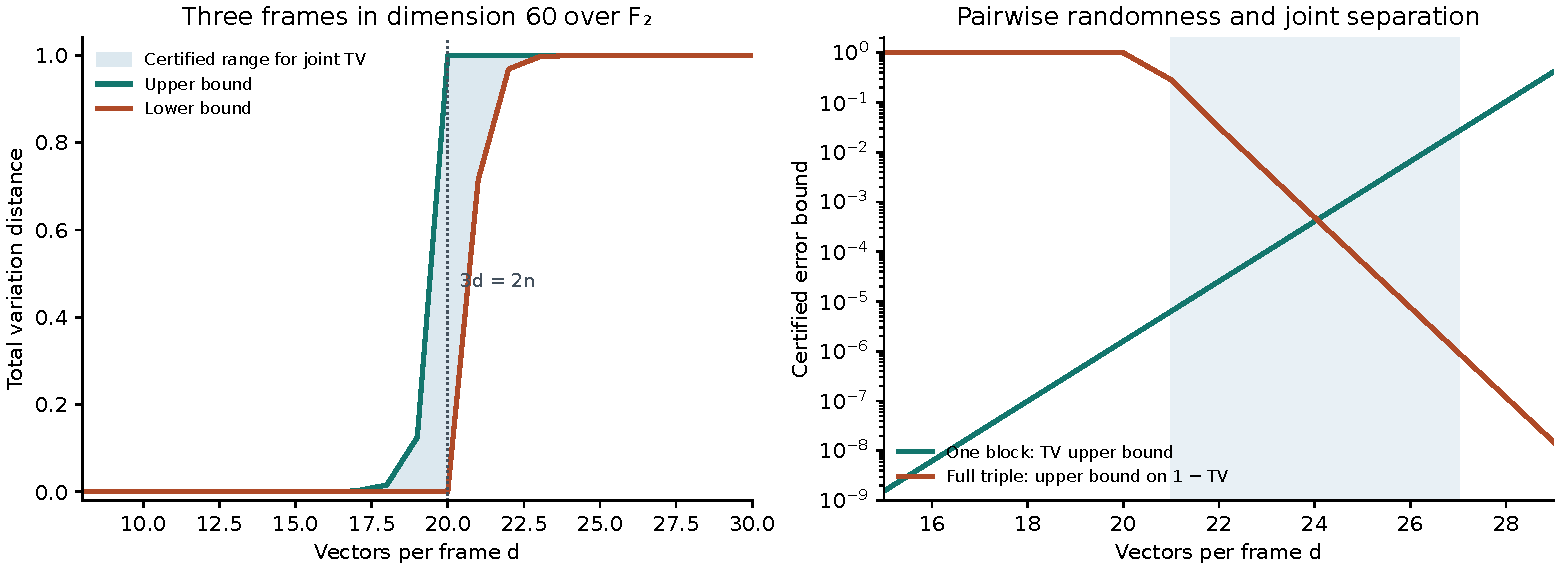
\includegraphics[width=\linewidth]{figures/dimension_threshold.pdf}
\caption{Certified bounds for three isotropic frames over $\F_2$ with ambient dimension $60$. The left panel displays the allowable interval given by Theorem~\ref{thm:main}; it is not an empirical or exact TV curve. The right panel compares the one-block upper bound with the full-triple separation bound. In a substantial range, individual blocks are nearly uniform while the complete observation is nearly distinguishable. All plotted inputs are rational values from \texttt{results/certified\_envelopes.csv}.}
\label{fig:threshold}
\end{figure}

\section{Counting isometric frames}

For $j\ge0$ set
\[
 \eta_j=\prod_{a=1}^j(1-q^{-2a}),\qquad\eta_0=1,
 \qquad\eta_\infty=\prod_{a=1}^\infty(1-q^{-2a})>0.
\]
The infinite product is positive since $\sum_aq^{-2a}<\infty$.

\begin{lemma}[Embedding count]\label{lem:emb}
For a fixed alternating space of dimension $a$ and rank $2s$, the number of isometric injections into $V$ is
\begin{equation}\label{eq:emb}
 \Emb_n(a,s)=q^{2na-\binom a2}\frac{\eta_n}{\eta_{n-a+s}}
 \quad\hbox{if }0\le2s\le a,\ a-s\le n,
\end{equation}
and is zero otherwise. The symplectic group is transitive on these injections.
\end{lemma}

\begin{proof}
Split the source as a nondegenerate $2s$-space and a radical of dimension $h=a-2s$. The first summand can be embedded in
\[
 \frac{\abs{\Sp_{2n}(q)}}{\abs{\Sp_{2(n-s)}(q)}}
\]
ways: an isometric image of a fixed symplectic basis can be completed to an ambient symplectic basis, and its pointwise stabilizer is naturally isomorphic to the symplectic group of its orthogonal complement. The group order is
\[
 \abs{\Sp_{2m}(q)}=q^{m(2m+1)}\eta_m.
\]
This follows by successively choosing a nonzero first vector and a partner of pairing one, then continuing in the orthogonal complement.

Once the nondegenerate summand is fixed, its radical must be an independent isotropic $h$-frame in a $2(n-s)$-dimensional symplectic space. After $j$ vectors have been chosen, their common orthogonal space has $q^{2(n-s)-j}$ elements and their span has $q^j$ elements. Hence the number of choices is
\[
 \prod_{j=0}^{h-1}\bigl(q^{2(n-s)-j}-q^j\bigr).
\]
It is positive exactly when $h\le n-s$. Multiplying and simplifying gives \eqref{eq:emb}; its product factors have indices from $n-a+s+1$ through $n$. To obtain transitivity, extend the isotropic radical vectors to hyperbolic pairs in the complement and complete a symplectic basis. Two such completed bases are carried to each other by a symplectic transformation.
\end{proof}

\section{The exact law for any number of frames}

Fix a candidate observation $\Gamma$. Write
\[
 \rank\Gamma=2s,\quad R=\rad\Gamma,\quad r=\dim R=D-2s,
 \quad R_i=R\cap E_i,\quad t_i=\dim R_i.
\]
The spaces $R_i$ form a direct sum, even though their sum need not equal $R$. Let $T_\ell$ count the $\ell$-dimensional subspaces $L\le R$ such that $L\cap R_i=0$ for all $i$. Gaussian binomial coefficients are defined by
\[
 \qb ab=\prod_{j=0}^{b-1}\frac{q^{a-j}-1}{q^{b-j}-1}
 \quad(0\le b\le a),
\]
and are zero outside that range.

\begin{theorem}[Exact joint likelihood and relation spaces]\label{thm:exact}
The kernel counts are
\begin{equation}\label{eq:mobius}
 T_\ell=
 \sum_{0\le j_i\le t_i}
 (-1)^Jq^{\sum_i\binom{j_i}2}
 \left(\prod_i\qb{t_i}{j_i}\right)
 \qb{r-J}{\ell-J},\qquad J=\sum_i j_i.
\end{equation}
The probability of the particular observation $\Gamma$ is
\begin{equation}\label{eq:exact}
 \mu(\Gamma)=
 \frac{\displaystyle\sum_{\ell=0}^{r}T_\ell\Emb_n(D-\ell,s)}
 {\displaystyle\prod_i\Emb_n(d_i,s_i)}.
\end{equation}
Moreover, the $\ell$th summand divided by the same denominator is the joint probability of $\Gamma$ and an $\ell$-dimensional space of linear relations among the combined frame columns.
\end{theorem}

\begin{proof}
For a finite vector space $W$,
\begin{equation}\label{eq:mobius-identity}
 \sum_{U\le W}(-1)^{\dim U}q^{\binom{\dim U}2}
 =\begin{cases}1,&W=0,\\0,&W\ne0.\end{cases}
\end{equation}
Indeed, for $\dim W=t$, the sum is the specialization at $z=1$ of
\[
 \prod_{h=0}^{t-1}(1-q^h z)
 =\sum_{j=0}^t(-1)^jq^{\binom j2}\qb tjz^j,
\]
which follows by induction using the Gaussian-binomial recurrence.

Use \eqref{eq:mobius-identity} for each intersection $L\cap R_i$ and multiply the resulting indicators. On summing over all $\ell$-subspaces $L\le R$, choose $U_i\le R_i$ of dimension $j_i$. Their sum is direct and has dimension $J$, so the number of $L$ containing it is $\qb{r-J}{\ell-J}$. This proves \eqref{eq:mobius}.

A tuple of frames is a linear map
\[
 F:E\longrightarrow V,\qquad F(v_1,\ldots,v_k)=\sum_iX_i v_i,
\]
with $F^*\langle\cdot,\cdot\rangle=\Gamma$ and each restriction $F|_{E_i}$ injective. Necessarily $L=\ker F\le R$. The restriction conditions are precisely $L\cap R_i=0$. Conversely, each such $L$ and each isometric injection $E/L\hookrightarrow V$ determine one and only one tuple with kernel exactly $L$. The quotient has dimension $D-\ell$ and rank $2s$. Lemma~\ref{lem:emb} therefore counts its injections. Dividing the total count by the number $\prod_i\Emb_n(d_i,s_i)$ of independent frame tuples gives \eqref{eq:exact} and its refinement.
\end{proof}

For fixed individual forms the joint likelihood is thus a function of the $k+1$ integers $(s,t_1,\ldots,t_k)$. Consequently these integers retain all information needed for a likelihood-ratio test against $\nu$. This does not mean that the separate ranks of the cross blocks suffice.

\begin{corollary}[Efficient evaluation of the exact law]\label{cor:algorithm}
Write
\begin{equation}\label{eq:kernelpoly}
 P(z)=\prod_{i=1}^k\prod_{h=0}^{t_i-1}(1-q^h z)=\sum_J b_Jz^J.
\end{equation}
Then
\begin{equation}\label{eq:kernelpoly-T}
 T_\ell=\sum_{J=0}^{\ell}b_J\qb{r-J}{\ell-J}.
\end{equation}
After Gaussian elimination computes the invariants of $\Gamma$, all $T_\ell$ and its likelihood can be obtained with $O(D^2)$ arithmetic operations once $q^{2n}$ is available, with Gaussian coefficients tabulated by their recurrence. Including binary exponentiation costs $O(D^2+\log(n+1))$ operations. This counts exact arithmetic operations, not bit complexity.
\end{corollary}

\begin{proof}
Expand each factor group in \eqref{eq:kernelpoly} by the same binomial identity and collect the terms with total index $J$ in \eqref{eq:mobius}. There are at most $r$ linear factors. Their product, the Gaussian table, and the triangular sums in \eqref{eq:kernelpoly-T} each require $O(D^2)$ operations. In the ratio of symplectic group orders, cancel the common factors before evaluation, leaving at most $D$ factors. The required powers are obtained from $q^{2n}$ and an $O(D)$ table of powers of $q$. Embedding counts and the final sum then have the same or smaller arithmetic cost.
\end{proof}

\section{Exact feasibility and minimum ambient dimension}

\begin{theorem}[Simultaneous realization]\label{thm:support}
An alternating block matrix $\Gamma$ can be realized by maps injective on every $E_i$ into a $2n$-dimensional symplectic space if and only if
\begin{equation}\label{eq:support}
 s+\max_i t_i\le n.
\end{equation}
Its minimum possible symplectic ambient dimension is exactly $2(s+\max_i t_i)$. This statement does not presuppose that the individual forms have already been realized.
\end{theorem}

\begin{proof}
Let $L\le R$ be the kernel of a realization and put $\ell=\dim L$. Since $L\cap R_i=0$, dimension gives $\ell\le r-t_i$ for every $i$. Its quotient has dimension $D-\ell$ and rank $2s$, so Lemma~\ref{lem:emb} requires
\[
 n\ge D-\ell-s\ge D-r+\max_i t_i-s=s+\max_i t_i.
\]

Conversely, set $t=\max_i t_i$. Choose injections $f_i:R_i\hookrightarrow\F_q^t$. Since the $R_i$ form a direct sum, extend their sum to a map $f:R\to\F_q^t$, taking zero on a complement of their direct sum. One $f_i$ is surjective, so $f$ is surjective, also when $t=0$. Its kernel $L$ has dimension $r-t$ and meets every $R_i$ trivially. The quotient $E/L$ has rank $2s$ and radical dimension $t$. Embed its nondegenerate part as $s$ standard hyperbolic pairs and its radical as one vector from each of $t$ further hyperbolic pairs. This gives an injective realization in dimension $2(s+t)$; compose with the quotient map. Every original summand remains injective because $L\cap E_i=L\cap R_i=0$.
\end{proof}

The proof is constructive. It gives a direct algebraic procedure for finding a smallest ambient realization, without enumerating a symplectic group. If every $H_i$ is nondegenerate, then $R_i=0$ for all $i$, and feasibility simplifies to $\rank\Gamma\le2n$. With degenerate individual forms, the radical-intersection terms are essential.

\section{One exact kernel moment}

The uniform model $\nu$ is a random alternating matrix with prescribed diagonal blocks. Its full rank distribution is unnecessary for the threshold theorem.

\begin{lemma}[Rank of the evaluation map]\label{lem:eval}
Let $\mathcal W$ be the vector space of alternating matrices with zero diagonal blocks. For a nonzero $v=(v_1,\ldots,v_k)\in E$, the linear map
\[
 \mathcal W\longrightarrow E^*,\qquad B\longmapsto Bv
\]
has rank $D-d_i$ if only $v_i$ is nonzero, and rank $D-1$ if at least two components are nonzero. In the latter case its image is the annihilator of $v$.
\end{lemma}

\begin{proof}
For a single active component $v_i$, the $i$th output block is zero. Each other output block is a free vector, obtained independently by varying the cross matrix incident to $i$. This gives rank $D-d_i$.

For at least two active components, use the coordinate pairing to identify the cokernel. A vector $w$ annihilates all $Bv$ exactly when, for every $i<j$,
\begin{equation}\label{eq:outer}
 w_i v_j^{\mathsf T}-v_i w_j^{\mathsf T}=0.
\end{equation}
Choose two nonzero components $v_i,v_j$. Equality of the two rank-one outer products forces $w_i=\lambda v_i$ and $w_j=\lambda v_j$ for the same scalar $\lambda$. This includes the zero case: if one of these $w$ components is zero, the other is zero. Pairing one chosen active component with every remaining component in \eqref{eq:outer} forces $w_h=\lambda v_h$ for all $h$. Thus the cokernel is exactly the line spanned by $v$, and the rank is $D-1$. Alternation puts the image in the annihilator of $v$, which has this same dimension. No division by two occurs.
\end{proof}

\begin{lemma}[Exact first kernel moment]\label{lem:moment}
For the model $\nu$,
\[
 \E_\nu q^{\nul\Gamma}=A,
\]
with $A$ as in \eqref{eq:A}. If every $H_i=0$, this simplifies to
\begin{equation}\label{eq:isotropic-moment}
 A=q+1-q^{1-D}+q^{-D}\sum_i(q^{d_i}-1)(q^{d_i}-q).
\end{equation}
\end{lemma}

\begin{proof}
Count the vectors in the kernel in expectation:
\[
 \E_\nu\abs{\ker\Gamma}=\sum_{v\in E}\Prob_\nu(\Gamma v=0).
\]
The zero vector contributes one. If $v$ is supported in $E_i$, it can be in the kernel only if $v_i\in\rad H_i$. There are $q^{d_i-2s_i}-1$ such nonzero vectors. For each, Lemma~\ref{lem:eval} gives probability $q^{-(D-d_i)}$.

There are $q^D-1-\sum_i(q^{d_i}-1)$ vectors supported in at least two blocks. For each, the random off-diagonal evaluation is uniform in the annihilator of $v$. The fixed diagonal contribution also lies in that annihilator because $\sum_iH_i(v_i,v_i)=0$. Consequently the kernel probability is $q^{-(D-1)}$. Summing gives \eqref{eq:A}. Setting $s_i=0$ and simplifying gives \eqref{eq:isotropic-moment}. Finally the multi-block contribution is at most $q$, and the $i$th single-block contribution is at most $q^{2(d_i-s_i)-D}$, proving \eqref{eq:A-bound}.
\end{proof}

\section{Proof of the distributional threshold}

\subsection{Below the ambient dimension}

Retain only frame tuples whose combined map $F:E\to V$ is injective. They define a subprobability measure $\mu_0\le\mu$. Let $f_0=\mu_0/\nu$ and $f=\mu/\nu$. All observation probabilities under $\nu$ are positive, so these are ordinary finite densities and $f\ge f_0$ pointwise.

\begin{lemma}[Injective contribution to the likelihood]\label{lem:injective}
If $c=2n-D\ge0$ and $r=\nul\Gamma$, then
\begin{equation}\label{eq:injective-density}
 f_0(\Gamma)=\mathbf 1_{\{r\le c\}}
 \frac{\prod_i\eta_{n-d_i+s_i}}
 {\eta_n^{k-1}\eta_{(c-r)/2}}.
\end{equation}
The right side is defined to be zero when $r>c$, without evaluating the last denominator. Otherwise $r$ and $c$ have the same parity, so its last subscript is a nonnegative integer.
\end{lemma}

\begin{proof}
The $\ell=0$ term in \eqref{eq:exact} is $\Emb_n(D,s)/\prod_i\Emb_n(d_i,s_i)$, since $T_0=1$. Multiply by $q^B$ to divide by $\nu(\Gamma)$. The powers of $q$ in \eqref{eq:emb} cancel by \eqref{eq:B}. Since $D-2s=r$,
\[
 n-D+s=(2n-D-r)/2=(c-r)/2.
\]
The embedding count is zero exactly when $r>c$. An alternating matrix has even rank, hence $r\equiv D\equiv c\pmod2$.
\end{proof}

\begin{proof}[Proof of Theorem~\ref{thm:main}(i)]
The sequence $\eta_j$ decreases, and $0\le n-d_i+s_i\le n$. Therefore
\begin{equation}\label{eq:C-lower}
 C:=\frac{\prod_i\eta_{n-d_i+s_i}}{\eta_n^{k-1}}
 \ge\eta_n\ge\eta_\infty.
\end{equation}
When $r\le c$, put $m=(c-r)/2$. The elementary product inequality $\prod(1-u_j)\ge1-\sum u_j$, first for finite products and then by a limit, gives
\[
 f_0(\Gamma)\ge\frac{\eta_\infty}{\eta_m}
 =\prod_{j=m+1}^\infty(1-q^{-2j})
 \ge1-\frac{q^{-2m}}{q^2-1}
 =1-\frac{q^{r-c}}{q^2-1}.
\]
When $r>c$, parity implies $r-c\ge2$, so $q^{r-c}/(q^2-1)>1$. Thus the uniform pointwise bound
\begin{equation}\label{eq:likelihood-deficit}
 (1-f_0(\Gamma))_+\le\frac{q^{r-c}}{q^2-1}
\end{equation}
holds in both cases. It is essential that we bound the missing likelihood, rather than trying to approximate all contributions from dependent tuples separately. Using $f\ge f_0$ and Lemma~\ref{lem:moment},
\[
 \TV(\mu,\nu)=\E_\nu(1-f)_+
 \le\E_\nu(1-f_0)_+
 \le\frac{q^{-c}}{q^2-1}\E_\nu q^r
 =\frac{A}{q^2-1}q^{-c}.
\]
The trivial bound one completes \eqref{eq:upper}.
\end{proof}

\subsection{Above the ambient dimension}

\begin{proof}[Proof of Theorem~\ref{thm:main}(ii)]
Every actual observation is $F^{\mathsf T}JF$, so its rank is at most $2n$. If $w=D-2n>0$, its nullity is at least $w$. In the uniform model, Markov's inequality applied to $q^r-1\ge0$ gives
\[
 \Prob_\nu(r\ge w)\le\frac{\E_\nu(q^r-1)}{q^w-1}
 =\frac{A-1}{q^w-1}.
\]
Compare the probabilities of the event $r\ge w$ under the two laws. This proves \eqref{eq:lower} and the claimed test. Part (iii) was proved in Lemma~\ref{lem:moment}; Corollary~\ref{cor:threshold} follows immediately.
\end{proof}

The proof explains why the threshold can be obtained without a complete distribution for the invariants $(s,t_1,\ldots,t_k)$. Below it, a subprobability already supplies almost all of the uniform likelihood. Above it, one rank obstruction rejects almost all independent data.

\section{Exact forest independence and hidden dependence of every order}

\begin{theorem}[Forest observations are independent]\label{thm:forest}
Let $G$ be any forest on the frame labels $\{1,\ldots,k\}$. The matrix-valued random variables $\{M_{ij}:ij\in E(G),\ i<j\}$ are mutually independent under the actual frame model. This holds for arbitrary prescribed individual alternating forms and at every finite size.
\end{theorem}

\begin{proof}
Choose a leaf $i$ with neighbor $j$. Condition on all frames except $X_i$. The distribution of $M_{ij}$, or of its signed transpose if the indexing is reversed, does not depend on the realized value of $X_j$. Indeed, Lemma~\ref{lem:emb} makes any two possible $X_j$ symplectically conjugate, and applying that symplectic transformation to the independent uniform $X_i$ preserves its law. Therefore the conditional distribution of the leaf edge is its unconditional two-frame law. It is independent of all remaining frames and edges. Remove the leaf and iterate; isolated vertices have no observations.
\end{proof}

For three frames, every pair of the three edges is a forest. Their three matrices are therefore pairwise independent exactly. The theorem does not assert independence for a graph containing a cycle.

\begin{theorem}[Dependence invisible in every proper frame marginal]\label{thm:hierarchy}
Fix $q$ and $k\ge3$. Choose a real number
\begin{equation}\label{eq:alpha}
 \frac2k<\alpha<\frac2{k-1},
\end{equation}
and let all $k$ frames be isotropic of dimension $d=\lfloor\alpha n\rfloor$ in dimension $2n$. For all sufficiently large $n$ the frames are admissible. For every proper subset of frame labels, its complete collection of cross blocks has distance $O_{q,k,\alpha}(q^{-\varepsilon n})$ from independent uniform entries, for some $\varepsilon>0$. The full collection has distance
\[
 1-O_{q,k,\alpha}(q^{-\varepsilon n})
\]
from that model and also from the product of its own edge marginal laws.
\end{theorem}

\begin{proof}
For $k\ge3$, \eqref{eq:alpha} implies $\alpha<1$, so $d\le n$. A proper subset with $j\ge2$ frames has total dimension $jd\le(k-1)d$ and is balanced. Its subcritical gap is at least $[2-(k-1)\alpha]n$. Theorem~\ref{thm:main} therefore bounds its distance by
\[
 \frac{q+1+j}{q^2-1}q^{-[2-(k-1)\alpha]n}.
\]
A one-frame marginal has no cross blocks. The full observation has gap
\[
 kd-2n\ge(k\alpha-2)n-k,
\]
which tends to infinity linearly, so the supercritical bound applies. Any positive $\varepsilon$ smaller than both $2-(k-1)\alpha$ and $k\alpha-2$ gives the stated common exponential rate.

Finally, each edge marginal is exponentially close to uniform, as the $j=2$ case. The total variation distance between the product of its actual edge marginals and the product of uniform edge laws is at most the sum of the marginal distances. There are only $\binom k2$ edges. The triangle inequality preserves the full-law separation.
\end{proof}

The words ``proper frame marginal'' are deliberate: all observations involving a removed frame are discarded together. The theorem does not claim that deleting any single edge from the full observation always removes its distinguishing power.

\subsection{Proof and numerical evaluation of the binary example}

Set $q=2$, $n=50$, $d=40$. For two isotropic frames, \eqref{eq:isotropic-moment} gives
\[
 A_2=5-6\cdot2^{-40}+2\cdot2^{-80}<5.
\]
Their gap is $2n-2d=20$, so Theorem~\ref{thm:main} proves \eqref{eq:headline-one}. For three such frames,
\[
 A_3=3+3\cdot2^{-40}-9\cdot2^{-80}+4\cdot2^{-120}.
\]
The gap is $3d-2n=20$, and hence
\begin{equation}\label{eq:headline-rational}
 \TV(\mu,\nu)\ge
 1-\frac{2+3\cdot2^{-40}-9\cdot2^{-80}+4\cdot2^{-120}}{2^{20}-1}
 >0.99999809.
\end{equation}
These are exact rational comparisons; the unrounded lower bound is approximately $0.9999980926495482$. The forest theorem proves pairwise independence. If $P$ is the product of the actual edge laws, then
\[
 \TV(\mu,P)\ge\TV(\mu,\nu)-\TV(P,\nu)
 \ge\TV(\mu,\nu)-3\frac{A_2}{3\cdot2^{20}}>0.99999332.
\]
This proves Theorem~\ref{thm:headline}. With equal prior probabilities, the rank test identifies the model with success probability greater than $0.99999904$.

\subsection{A small exact illustration}

Sample three nonzero vectors independently and uniformly from $\F_2^2$. Their three pairings are bits with distribution
\begin{center}
\begin{tabular}{@{}cccccc@{}}
\toprule
Output & $000$ & $011$ & $101$ & $110$ & $111$\\
\midrule
Probability & $1/9$ & $2/9$ & $2/9$ & $2/9$ & $2/9$\\
\bottomrule
\end{tabular}
\end{center}
The other three outputs have probability zero. A zero pairing means that the two nonzero vectors are equal. Thus $000$ comes from the three equal triples; each other listed output comes from six triples. Each bit is Bernoulli with parameter $2/3$, and any two bits are independent, although the three are not. Their exact distance from three independent fair bits is $7/18$. The large example strengthens the phenomenon by making the marginal biases negligible and the full separation nearly maximal.

\section{Verification, reuse, and remaining questions}

\subsection{Exact computational checks}

The script \texttt{code/exhaustive\_check.py} independently enumerates frame tuples over prime fields and compares their observed frequencies with \eqref{eq:exact}. It uses exact integer and rational arithmetic. It checks all possible observations, including impossible ones, rather than sampling only realized outputs.

\begin{center}\small
\begin{tabular}{@{}rrllrr@{}}
\toprule
$q$ & $n$ & $(d_i)$ & $(2s_i)$ & Tuples & Exact TV\\
\midrule
2&1&$(1,1,1)$&$(0,0,0)$&27&$7/18$\\
2&1&$(1,1,1,1)$&$(0,0,0,0)$&81&$25/32$\\
3&1&$(1,1,1)$&$(0,0,0)$&512&$2/9$\\
2&2&$(2,1,1)$&$(0,0,0)$&20,250&$269/2400$\\
2&2&$(1,1,1,1)$&$(0,0,0,0)$&50,625&$4061/36000$\\
2&2&$(2,2,1)$&$(0,0,0)$&121,500&$6463/19200$\\
3&2&$(1,1,1)$&$(0,0,0)$&512,000&$71/3600$\\
2&2&$(2,1,1)$&$(2,0,0)$&27,000&$19/160$\\
3&1&$(2,1,1)$&$(2,0,0)$&1,536&$179/243$\\
\bottomrule
\end{tabular}
\end{center}

Across these nine cases, all $733{,}531$ frame tuples and all $753$ possible Gram observations were accounted for. The exact likelihood, support criterion, moment, and stated TV bounds agreed in every case. All $83$ nontrivial forest marginals checked were independent. A second likelihood implementation, \texttt{code/exact\_law.py}, uses the polynomial formula \eqref{eq:kernelpoly-T} and agrees with all $753$ observations. A separate moment enumerator checks $60{,}685$ matrices in $23$ form configurations, including every individual rank pattern for three two-dimensional blocks over $\F_2$.

These finite tests support the implementations and detect sign, normalization, and characteristic-two errors. The all-dimensional claims are established by the proofs in this paper, not by extrapolation from the tests.

\subsection{Reproducing the packet}

The core verification and likelihood programs use Python's standard library. The figure program additionally uses Matplotlib. Run from the packet directory:
\begin{verbatim}
python3 code/exhaustive_check.py
python3 code/independent_moment_check.py
python3 code/exact_law.py --q 2 --n 50 --dimensions 40 40 40
python3 code/make_figure.py
pdflatex -interaction=nonstopmode -halt-on-error paper.tex
pdflatex -interaction=nonstopmode -halt-on-error paper.tex
\end{verbatim}
Formula evaluation accepts prime-power field sizes. The supplied matrix-rank and exhaustive routines work over prime fields; they do not treat arithmetic modulo $p^a$ as arithmetic in $\F_{p^a}$.

The archive contains the complete LaTeX source, compiled PDF, figure, exact data, a source and novelty audit, and a formalization plan. No Lean-checked theorem is claimed for this new result. The formalization plan separates linear algebra, finite counting, and the probability estimates so that the proof can be integrated into the existing project without importing an analytic GRH theorem.

\subsection{What remains open}

The present bounds leave the fixed-gap profile $D-2n=O(1)$ unresolved for general frame types. The exact likelihood supplies a finite algorithm but does not by itself enumerate how many observations have each invariant tuple. Determining these distributions would yield the exact critical profile and finite-size optimal tests. Other natural questions are the distinguishing power of sparse observation graphs containing cycles, versions over finite local rings, and nonuniform symplectic sampling. The forest theorem and the rank test establish two endpoints for the graph question; they do not classify all intermediate graphs.

\begin{thebibliography}{9}
\bibitem{ProveIt}
V. Reshetnikov and contributors, \emph{ProveIt: Generalized Riemann Hypothesis research directory}, snapshot \texttt{6d284fcf75bc3a91bb2e79ba7636f94724bff62c}, 27 November 2026.
\href{https://github.com/VladimirReshetnikov/ProveIt/tree/6d284fcf75bc3a91bb2e79ba7636f94724bff62c/Analysis/GeneralizedRiemannHypothesis}{Pinned project directory}.
In particular, \href{https://github.com/VladimirReshetnikov/ProveIt/blob/6d284fcf75bc3a91bb2e79ba7636f94724bff62c/Analysis/GeneralizedRiemannHypothesis/Article/sections/spn.tex}{the frame-statistics section}, labels \texttt{spn:thm:complete-law} and \texttt{spn:q:symplectic}; the incoming reports \emph{Uniform rank blindness in rectangular symplectic blocks}, \emph{Uniform rank and joint-defect laws for rectangular symplectic blocks}, and \emph{Two open questions from the ProveIt GRH article}.

\bibitem{Sutherland}
Andrew V. Sutherland, \emph{Verification files for the shorter Lean proof of RH and of GRH for Dirichlet L-functions}, updated 27 November 2026, 17:27 UTC.
\url{https://math.mit.edu/~drew/shortgrh/}.

\bibitem{FulmanGoldstein}
Jason Fulman and Larry Goldstein, \emph{Stein's method and the rank distribution of random matrices over finite fields}, Annals of Probability \textbf{43} (2015), 1274--1314.
\href{https://doi.org/10.1214/13-AOP889}{doi:10.1214/13-AOP889}.

\bibitem{LiEtAl}
Tiange Li, Yinan Li, Youming Qiao, Dacheng Tao and Yingjie Wang,
\emph{On the average-case complexity landscape for Tensor-Isomorphism-complete problems over finite fields}, arXiv:2604.00591v2, 3 November 2026. Proposition 5.2 and Section 6.4.1.
\url{https://arxiv.org/abs/2604.00591}.

\bibitem{Farshi}
Tom Farshi, Daniele Toniolo, Carlos E. Gonz\'alez-Guill\'en, \'Alvaro M. Alhambra and Lluis Masanes,
\emph{Mixing and localization in random time-periodic quantum circuits of Clifford unitaries}, Journal of Mathematical Physics \textbf{63} (2022), 032201.
\href{https://doi.org/10.1063/5.0054863}{doi:10.1063/5.0054863}; \href{https://arxiv.org/abs/2007.03339}{arXiv:2007.03339}.

\bibitem{He}
Jimmy He, \emph{Random walk on the symplectic forms over a finite field}, Algebraic Combinatorics \textbf{3} (2020), 1165--1181.
\href{https://doi.org/10.5802/alco.131}{doi:10.5802/alco.131}.
\end{thebibliography}
\end{document}
